\section{Additional Experimental Details for LLM Training}

\subsection{Pretraining Setup}\label{app:setup}

% \paragraph{Pretraining Setup.}
In our pretraining experiments, we employ the AdamW optimizer with a weight decay of 0.1 and a gradient clip of 1.0. We set the peak learning rate to 0.001, aligning with the approximate optimal learning rate reported by~\citet{li2025predictablescalei}. Balancing the optimal batch size suggested by~\citet{li2025predictablescalei} with training efficiency, we utilize a sequence batch size of 128, which corresponds to roughly 0.5M data points per batch. We adopt the vocabulary of Qwen2.5~\citep{qwen2025qwen25technicalreport} models. Our pretraining model consists of approximately 117 million non-embedding parameters, consistent with the methodology of~\citet{kaplan2020scaling}, and a total of 331 million parameters following the convention of~\citet{hoffmann2022training}. The detailed hyperparameter configurations are presented in \Cref{tab:hyper}, and the model architecture specifications are provided in \Cref{tab:model}. To ensure a fair comparison by eliminating the influence of batch order variations, we fix the random seed that governs the data stream across all experiments.

% \begin{figure}
%     \centering
%     % \includegraphics[width=0.6\linewidth]{figs/loss_over_step.pdf}
%     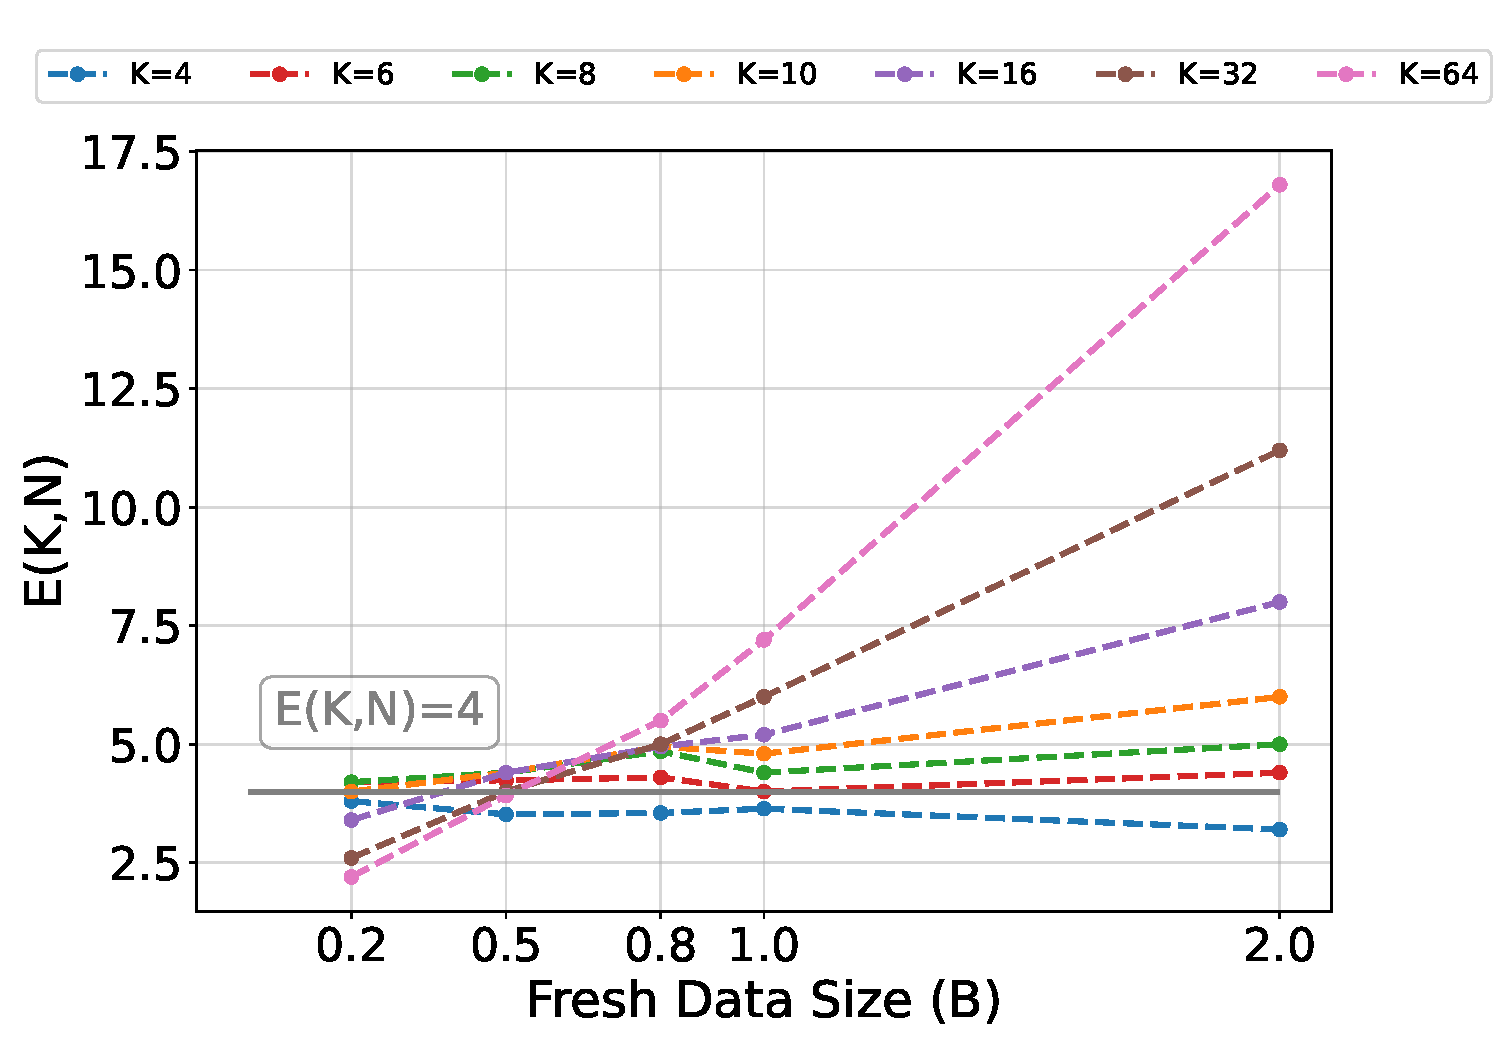
\includegraphics[width=0.6\linewidth]{figs/E_k_over_fresh_data_size.pdf}
    
%     \caption{The effective reuse rate $E(K,N)$ as a function of the fresh data size $N$.}\label{fig:ek-data}
% \end{figure}
%     % \includegraphics[width=\linewidth]{figures/LLM/loss_over_step.pdf}
%     % \caption{Training loss as a function of training steps for different fresh data sizes.}
%     % \label{fig:loss-step}

    
\begin{table}[htbp!]
\centering
\caption{Model configurations and parameter counts. $d_h$: hidden dimension; $d_f$: feed-forward dimension; $n_l$: number of Transformer layers; $n_h$: number of attention heads; $n_{kv}$: number of key-value heads (for grouped-query attention); Vocab Size: size of tokenizer vocabulary; \#NE params: number of non-embedding parameters (in millions); \#Params: total number of model parameters (in millions).}
\label{tab:model}
\begin{tabular}{lrrrrrrrrr}
\toprule
Name & $d_{h}$ & $d_f$ & $n_l$ & $n_h$ & $n_{kv}$ & Vocab Size & \#NE params & \#Params \\
\midrule
0.5B & 896 & 4864 & 24 & 14 & 2 & 151936 & 355 & 491 \\
0.3B & 640 & 3328 & 16 & 10 & 2 & 151936 & 117 & 331 \\
\bottomrule
\end{tabular}
\end{table}


\begin{table}[htbp!]
\centering
\caption{LLM Experiment Settings\label{tab:hyper}}
\begin{tabular}{ll}
\toprule
\textbf{Parameter} & \textbf{Value} \\
\midrule
\textbf{Data} & \\
\quad Sequence Batch Size & 128 \\
\quad Sequence Length & 4096 \\
\midrule
\textbf{Learning Rate} & \\
\quad Peak Learning Rate & 0.001 \\
\quad Schedule & Constant \\
\quad Warmup Steps & 400 \\
\midrule
\textbf{Optimizer} & \\
\quad Optimizer & AdamW \\
\quad Weight Decay & 0.1 \\
\quad $\beta_1$ & 0.9 \\
\quad $\beta_2$ & 0.95 \\
\quad $\epsilon$ & 1e-8 \\
\quad Gradient Clip & 1.0 \\
\bottomrule
\end{tabular}
\end{table}

% \section{Additional Experiments}\label{app:setup}

% In our pretraining experiments, we employ the AdamW optimizer with a weight decay of 0.1 and gradient clip of 1.0. We choose the peak learning rate as 0.001, around the optimal learning rate reported in~\citet{li2025predictablescalei}. We trade-off the optimal batch size according to~\citet{li2025predictablescalei} with the training efficiency, and use sequence batch size as 128, approximately 0.5M data each batch. Our pretraining model is approximately 117M when accounting non-embedding parameters conforming to~\citet{kaplan2020scaling} practice and 331M in total when following~\citet{hoffmann2022training} practice. Hyperparameter configurations are listed in \Cref{tab:hyper}, and detailed model architecture specifications are provided in \Cref{tab:model}. To ensure a fair comparison by eliminating the impact of batch order variations, we fix the random seed governing the data stream across all experiments. 

% \begin{table}[htbp!]
% \centering
% \caption{Model configurations and parameter counts. $d_h$: hidden dimension; $d_f$: feed-forward dimension; $n_l$: number of Transformer layers; $n_h$: number of attention heads; $n_{kv}$: number of key-value heads (for grouped-query attention); Vocab Size: size of tokenizer vocabulary; \#NE params: number of non-embedding parameters (in millions); \#Params: total number of model parameters (in millions).}
% \label{tab:model}
% \begin{tabular}{lrrrrrrrrr}
% \toprule
% Name & $d_{h}$ & $d_f$ & $n_l$ & $n_h$ & $n_{kv}$ & Vocab Size & \#NE params & \#Params \\
% \midrule
% 0.5B & 896 & 4864 & 24 & 14 & 2 & 151936 & 355M & 491M\\
% 0.3B & 640 & 3328 & 16 & 10 & 2 & 151936 & 117M & 331M\\
% \bottomrule
% \end{tabular}
% \end{table}


% \begin{table}[h!]

% \centering

% \caption{LLM Experiment Settings\label{tab:hyper}}

% \begin{tabular}{ll}

% \toprule

% \textbf{Parameter} & \textbf{Value} \\

% \midrule

% \textbf{Data} & \\

% \quad Sequence Batch Size & 128 \\

% \quad Sequence Length & 4096 \\

% \midrule

% \textbf{Learning Rate} & \\

% \quad Peak Learning Rate & 0.001 \\

% \quad Schedule & Constant \\

% \quad Warmup Steps & 400 \\

% \midrule

% \textbf{Optimizer} & \\

% \quad Optimizer & Adam \\

% \quad Weight Decay & 0.1 \\

% \quad $\beta_1$ & 0.9 \\

% \quad $\beta_2$ & 0.95 \\

% \quad $\epsilon$ & 1e-8 \\

% \quad Gradient Clip & 1.0 \\

% \bottomrule

% \end{tabular}

% \end{table}
\subsection{Fitting Experiments} \label{app:fitting experiments}
To provide real-world evidence that larger datasets can be repeated more, we show how the saturation points can be used to determine the appropriate number of training epochs. Recall that the saturation points are the points at which multi-epoch training first starts to underperform the one-pass baseline. We estimate these points from the pretraining loss curves presented in \Cref{sec:experiment-llm} and fit its dependence on $N$. 
% This fitted relationship provides an empirical rule for determining how many passes to use for a given dataset size: one can plug in this dataset size into the fitted formula and calculate $E(K,N)$. It represents a balance between training efficiency and low validation loss, thus its value is the suggested number of epochs.


To estimate this quantity from the training curves, we proceed as follows. First, to reduce the impact of noise, we smooth the loss curves with exponential moving average (EMA) with decay coefficient $\alpha = 0.9$ and a window size of 3 checkpoints. Then for each dataset size $N$, we examine the ratio $E(K,N)/K$. A larger ratio requires multi-epoch training to remain very close to the one-pass baseline, whereas a smaller ratio allows more deviation. Next, given a threshold hyperparameter $\lambda$, we identify the closest epoch $K$ at which this ratio first falls below $\lambda$, which we denote as $K(\lambda, N)$. Here we choose $\lambda = 0.75$, and we define $K(\lambda, N)$ as the saturation point.
% Finally, we take the corresponding $E(K,N)$ as the saturation point, and we denote this as $K(\lambda,N)$.

We fit those points and find that $K(\lambda,N)\approx 0.80\log N + 5.21$ with a correlation coefficient of $r=0.97$. The fitting results are shown in \Cref{fig:ek-n-saturation point}. 

% \subsection{Experiments on Learning Rate Schedule} \label{app:experiment-llm-lrs}
% Next, we conduct experiments to find how different learning rate schedules affect our experiment results. Here we select a $2$-stage learning rate schedule. Specifically, we first load checkpoints of our experiments with fresh dataset size 0.2B, 0.5B, 1B, 2B in \Cref{sec:experiment-llm} when trained for $2, 4, 8, 16$ epochs, and perform a linear learning rate decay from $10^{-3}$ to $10^{-5}$ for one epoch. For one-pass scenario, we take a learning rate schedule same as that of 2B. Then, for each dataset size, we fit the final loss after the decay, and fit a loss curve using the formula $y = A + \frac{B}{x^a}$. The fitted curves are used to predict the final loss after such a learning rate schedule. Finally, we use the curves to predict $E(K,N)$.

% Our results can be seen in \Cref{fig:ek-n-saturation-point-lrs}. We can see that under a different learning rate schedule, we still observe that $E(K,N) = \Theta(\log N)$. Specifically, we have $E(K,N)\approx 2.35\log N + 5.25$ with a coefficient of $0.96$. This shows that larger datasets can be repeated more under different learning rate schedules.
\begin{figure}[t]
    % \vspace{-0.4in}
    \centering
    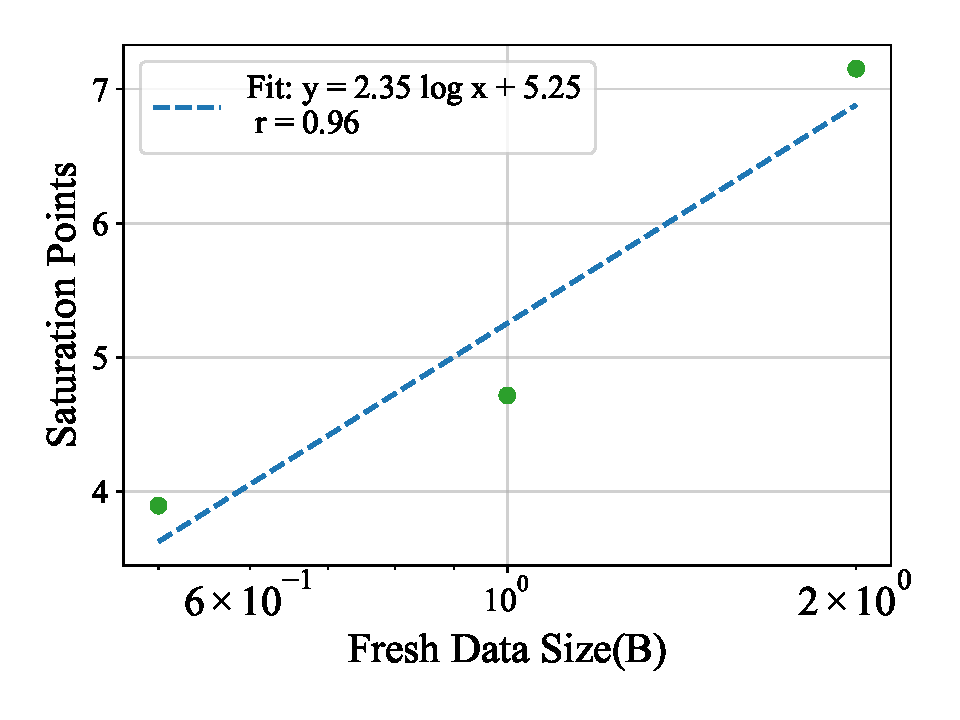
\includegraphics[width=0.5\linewidth]{figs/E_KN_vs_N_lrs.pdf}
    \caption{The saturation points $K(\lambda, N)$ as a function of the data size $N$ under a WSD learning rate schedule with linear decay.}
    \label{fig:ek-n-saturation-point-lrs}
\end{figure}
\subsection{Experiments with WSD Learning Rate Schedule}
\label{app:experiment-llm-lrs}

Next, to make our LLM experiments more consistent with real-world pretraining practices, we repeat the LLM experiments under a warmup-stable-decay(WSD) learning rate schedule.

Concretely, we start from the checkpoints obtained in \Cref{sec:experiment-llm} for fresh data sizes
$N \in \{0.2\text{B}, 0.5\text{B}, 1\text{B}, 2\text{B}\}$ after $K \in \{2,4,8,16\}$ epochs of pretraining with a constant learning rate of $10^{-3}$. From each checkpoint, we continue training for one additional epoch while linearly decaying the learning rate from $10^{-3}$ to $10^{-5}$, resulting in a WSD learning rate schedule followed by a linear decay. For the one-pass baseline, we adopt the same schedule as in the $N=2\text{B}$ run.

For each dataset size $N$, this process produces a set of four validation-loss values, each associated with one of the four selected epoch numbers $K$. We model the dependence of the final loss on the training steps $x$ using the parametric form  $\ell(x) = A + \frac{B}{x^{a}}$, where $A,B,a$ are fitted parameters. The fitted curves are then used to predict the final validation loss under this WSD schedule for arbitrary training budgets. Using these predictions, we compute the saturation points following the same procedure as in \Cref{sec:experiment-llm}. Here we still choose $\lambda = 0.75$.

The resulting saturation points are summarized in \Cref{fig:ek-n-saturation-point-lrs}. We observe that, even under this different learning rate schedule, the saturation points still satisfy the logarithmic scaling $K(\lambda,N) = \Theta(\log N).$ Specifically, we have $K(\lambda,N) \approx 2.35 \log N + 5.25$ with a correlation coefficient of $r = 0.96$. This confirms that our message that larger datasets can be repeated more also holds for real LLM training setups.
